%!TEX root = documentation.tex

\chapter{Master}

\section{About the Master} % (fold)
\label{sec:about_the_master}
The master is written in Java and uses the jamod Library\footnote{\url{http://jamod.sourceforge.net/}} for the communication with the slaves using the Modbus protocol. The view is created with the SWT Library\footnote{\url{http://www.eclipse.org/swt/}}. 

Before the collection process of the measurement values can be started it's necessary to create a configuration. In this configuration all slaves are defined. A slave must be added to the master before it can be used. Each slave has an individual name and IP address. In the configuration phase it's necessary to specify the kind of data the slaves collect. The data that is transferred from the slave to the master is called Input Parameter. To configure the sensor, it's possible to define Configuration Parameters. These values are transferred from the master to the slave. To map the parameters to the memory in the slave, they must be bound to addresses. This happens individually for each slave. So it's possible to collect different sensor data from different slaves. It's also possible to configure the kind of plots that are generated (see Section \ref{sub:plots}).

After the configuration of the slaves the collection process can be started. While each slave is polled in its own thread, a single collector thread collects the data, generates a text file with the information about the current values and draws the plots. The time between polling of the slaves and generation of the output files can also be configured. As soon as the current day changes the values from the last day are aggregated to a history value. The values from the slave are kept for two days so it's possible to build a plot based on hourly data from the last day. 

% section about_the_master (end)
\section{Implementation} % (fold)
\label{sec:implementation}
The source code can be downloaded at github\footnote{\url{http://www.github.com/schugabe/fws}}. The doc folder\footnote{\url{http://github.com/schugabe/FWS/tree/master/master/FWS_Master/doc/}} contains the javadoc generated source code documentation. In the following list a short overview on the classes and their functionality is provided. For a class diagram, see Figure \ref{fig:class_master}.

\begin{itemize}
    \item Configuration: Parameter, InputParameter, ConfigParameter, SlaveInputBinding, SlaveConfigBinding, Slave
    \item Save the configuration: PersistencePreferences, all classes with ContentHandler in their name
    \item Data collection: Slave, MeasurementCollector, Measurement, SlaveInputBinding, MeasurementHistoryController, MeasurementHistory, MeasurementHistoryEntry
    \item Plotting and Output generation: MeasurementCollector, PlotBase, TimePlot, CurrentPlot
    \item ModBus: ModbusWrapper, Slave
    \item View: All classes that start with view (not shown in class diagram)
\end{itemize}

\begin{figure}[H]
    \centering
    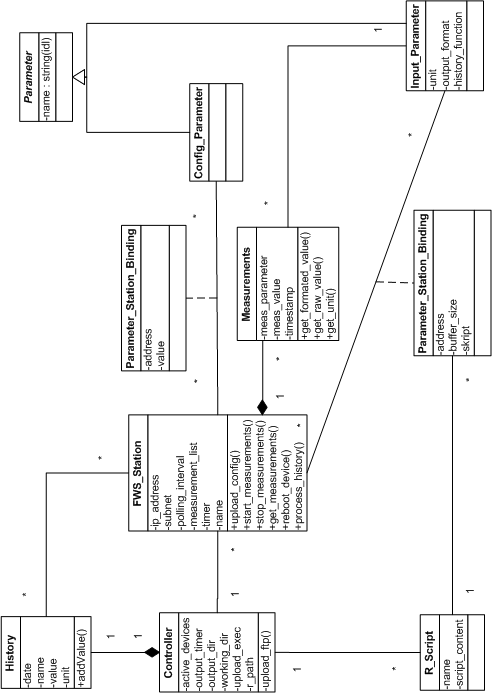
\includegraphics[width=\linewidth]{master/class.png}
    \caption{Class diagram of the master}
    \label{fig:class_master}
\end{figure}

% section implementation_details (end)

\section{Configuration} % (fold)
\label{sec:configuration} 

The views that support the configuration are shown in Figures \ref{fig:add}, \ref{fig:settings}, \ref{fig:parameter} and \ref{fig:slaves}.

The result of the configuration phase is an XML file with all settings in it (Listing \ref{code:settings}). The location of this file is OS dependent. 
\begin{itemize}
    \item \textbf{OS X}: /Users/\{username\}/Library/Application Support/FWSMaster/settings.xml
    \item \textbf{Linux}: \textasciitilde /.fws\_master/settings.xml
    \item \textbf{Windows}: C:\textbackslash \{User Dir\} \textbackslash .fws\_master \textbackslash settings.xml
\end{itemize}

{\C \lstinputlisting[language=xml,breaklines=true,caption={Sample settings file},label=code:settings,frame=tlRB]{master/settings.xml} }

\subsection{Parameters} % (fold)
\label{sub:parameters}
There are two types of parameters. Input Parameters and Configuration Parameters. Each parameter has a unique name and a boolean value if it's enabled. The name is the identifier of the parameter so it has to be unique. Beside of these common attributes the Configuration and Input Parameters have further attributes. The parameters must be assigned to slave addresses. This process is referred to as binding a parameter to a slave. To bind a parameter to a slave, the user must define the address on the slave where the parameter is saved.

\subsubsection{Input Parameter} % (fold)
\label{ssub:input_parameter}
Additional attributes of an Input Parameter:
\begin{itemize}
	\item Unit
	\item Format
	\item History Function
\end{itemize}

\paragraph{Unit} % (fold)
\label{par:unit}
The unit is just used for the description in the generated files. Available units are:
\begin{itemize}
	\item speed $\frac{m}{s}$
	\item speed $\frac{km}{h}$
	\item frequenzy $Hz$
	\item direction
	\item temperature $^\circ C$
\end{itemize}

% paragraph unit (end)

\paragraph{Format} % (fold)
\label{par:format}
The transferred value from the slave is a 16 bit integer value. To be able to display floating point numbers, it's possible to set the desired output format. Example: The temperature equals $23.3 ^\circ C$. The slave measures the temperature and converts it to $233$. This integer value is then transmitted to the master. The master converts the number back to the desired format. 

\paragraph{History Function} % (fold)
\label{par:histfunc}
There are three different history functions available. For more details about these functions and how they are used refer to Section \ref{sec:history}.
\label{par:history_function}
\begin{itemize}
    \item average
    \item minimum
    \item maximum
\end{itemize}
% paragraph history_function (end)
% paragraph format (end)
% subsubsection input_parameter (end)

\subsubsection{Configuration Parameter} % (fold)
\label{ssub:configuration_parameter}
Additional attributes of a Configuration Parameter:
\begin{itemize}
    \item value
\end{itemize}

\paragraph{Value} % (fold)
\label{par:value}
A configuration parameter is a value that is transferred from the master to the slave. The value transferred is saved in the attribute value. This value must be a 16 bit integer value.
% paragraph value (end)
% subsubsection configuration_parameter (end)

% subsection parameters (end)

\subsection{Plots} % (fold)
\label{sub:plots}
The plots are generated with the help of the jFreeChart Library \footnote{\url{http://www.jfree.org/jfreechart/}}.
The plots can be particularly configured for the input parameters. Each binding can have several plots assigned. It's also possible to plot more than one data into one plot. The plots are configured with a string. The simplest configuration looks like {\C h24;} With that configuration one plot is generated and the data for this plot are the values from the last 24 hours. The plots are generated in the output directory that can be set by the user.

It's possible to use different data ranges for the plots. To allow the user to choose one range there are three different time bases available:
\begin{itemize}
	\item c - current
	\item h - hours
	\item d - days
\end{itemize}

\paragraph{Current} % (fold)
\label{par:current}
represents the newest values for the plot. Currently this is only implemented for the wind direction. Figure \ref{fig:current} provides an example.
\begin{figure}[ht]
    \centering
    
\includegraphics[width=0.9\linewidth]{master/plot_examplec.png}
    \caption{Current wind direction plot}
    \label{fig:current}
\end{figure}
% paragraph current (end)

\paragraph{Hours} % (fold)
\label{par:hours}
represents the values of the last hours for the plot. The amount of the hours is specified in the plot configuration. It's the number after the timebase. Figure \ref{fig:hours} provides an example of a 24 hour plot.
\begin{figure}[ht]
    \centering
    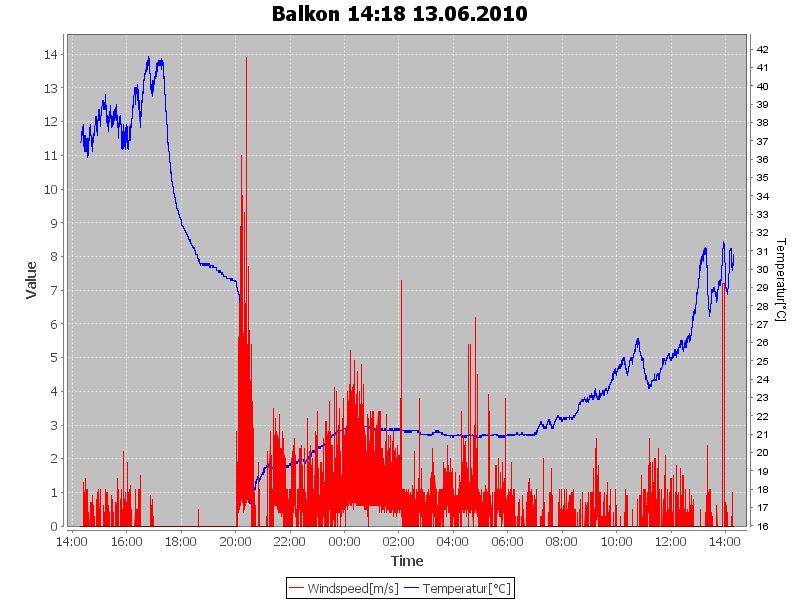
\includegraphics[width=0.9\linewidth]{master/plot_exampleh.png}
    \caption{Last 24 hours of two separate parameters in one plot}
    \label{fig:hours}
\end{figure}
% paragraph hours (end)

\paragraph{Days} % (fold)
\label{par:days}
plots the values from the last days. For more details about the history, see Section \ref{sec:history}.
% paragraph days (end)

\subsubsection{Configuration Syntax} % (fold)
\label{ssub:configuration_syntax}
Each plot is specified by three different parts: [Number]CharacterNumber;

\paragraph{First Number} % (fold)
\label{par:first_number_id}
This number is optional and controls if more than one input parameter is drawn in one plot. All configured plots with the same first number (ID) are drawn in the same plot.
% paragraph first_number_id (end)
\paragraph{Character} % (fold)
\label{par:character}
Defines the timebase.
% paragraph character (end) 
\paragraph{Second Number} % (fold)
\label{par:number}
The second number defines how much data will be in the plot (amount of data). {\C d4;} will plot the last four days.
% paragraph number (end)
\paragraph{End of Configuration} % (fold)
\label{par:end_of_configuration}
Each configuration must end with an {\C `;'}.
% paragraph end_of_configuration (end)

\paragraph{Example} % (fold)
\label{par:example}
For the configuration string {\C h24;1h24;d30;c1;d365;} the following plots are generated:
\begin{itemize}
	\item Last 24 hours
	\item Last 24 hours with other data with ID 1 
	\item Last 30 days
	\item Current value
	\item Last 365 days
\end{itemize}

% paragraph example (end)
% subsubsection configuration_syntax (end)

\subsubsection{Detailed Information about the plots} % (fold)
\label{ssub:detailed_information_about_the_plots}
If two different datasets are plotted in one diagram two axes with separate scales will be generated. When more than two data sets should be drawn in one diagram they share one axis.

The direction parameters values are not connected with a line. Otherwise the diagrams would get unreadable if the wind direction changes a lot.

The direction parameter values are mapped to a description of the direction. $0^\circ$ results in N(orth) (see Figure \ref{fig:dir})

\begin{figure}[ht]
    \centering
    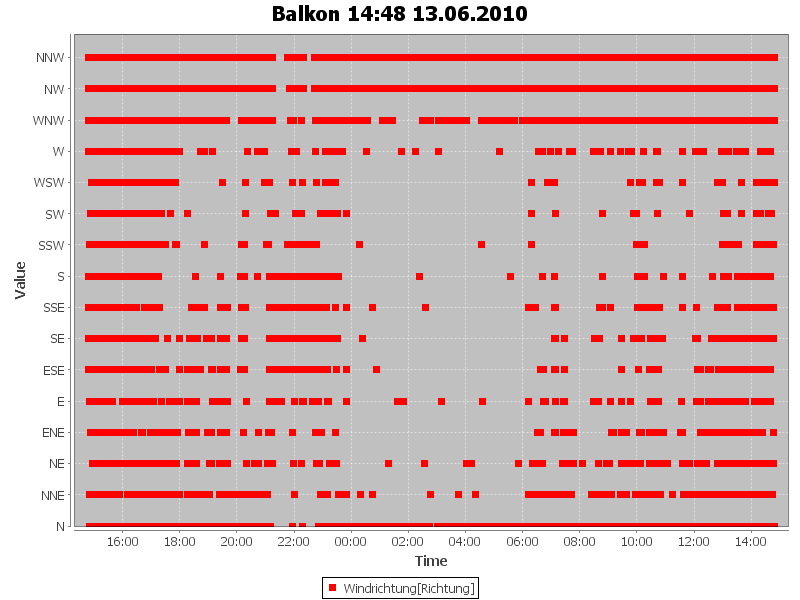
\includegraphics[width=0.9\linewidth]{master/plot_dir.png}
    \caption{Axis description of direction parameter}
    \label{fig:dir}
\end{figure}
% subsubsection detailed_information_about_the_plots (end)
% subsection plots (end)
% section configuration (end)

\section{Slaves} % (fold)
\label{sec:slaves}

After the slaves are configured they are added to the slave controller. This controller takes care for starting and pausing the specific threads. 

\subsubsection{Transferring the Data} % (fold)
\label{ssub:getting_the_data}
Each slave has its own thread assigned. This thread polls in its own interval the data values from the slave. For each transmission a new TCP connection is opened. After the value has been transferred the connection gets closed. This is necessary as the TCP stack of the slave doesn't support keep alive signals. Leaving the connection open would otherwise result in timeouts. Each slave has a list of measurements. A measurement consists of a timestamp and a value. These lists are collected from the Output Generation thread. If a slave is paused its thread gets suspended and waits for the wake up signal from the controller. 

The Modbus function that is used to transfer the data is named sendReadRequest.
% subsubsection getting_the_data (end)

\subsubsection{Transferring the configuration} % (fold)
\label{ssub:transferring_the_configuration}
When the user wants to upload a new configuration the slave will call the method sendWriteRequest for each Configuration Parameter and reads back the answer of the slave. If the answer equals the previously sent value the value is marked as transferred. A transferred value isn't uploaded again if it is unchanged.
% subsubsection transferring_the_configuration (end)
\subsubsection{Change the IP Address} % (fold)
\label{ssub:change_the_ip_address}
The IP Address represents a special configuration parameter. It is always mapped to the address 0 and 1 on the slave. These two 16 bit registers are used to save the IP address. When the IP address has been changed it's transferred to the slave. After the successful transmission of the two values the new IP is saved. Otherwise the old IP is kept.
% subsubsection change_the_ip_address (end)


\subsubsection{Collecting the Data} % (fold)
\label{ssub:collecting_the_data}
A data collector thread runs in background an collects the data from all the slaves. For each slave/parameter combination a distinct list is kept with all the recent values in it. Before saving the measurements they are converted into a simpler data type that can be serialized and does not have references to other classes.

In the collector thread the text file is generated that contains the information about the current status of the slaves. Each slave is represented in this file. The information written in this file are the current values of the Input Parameters bound to that slave. This value is the average of the measurements since the last run of the collector. To be able to see how the value changed the standard deviation is calculated and written to the output. An example of a result file is given in Listing \ref{code:result}. 
For each parameter a new line is started in the file. The syntax is {\C name[unit]:value;standard deviation;}

{\C \lstinputlisting[breaklines=true,caption={Sample result file},label=code:result,frame=tlRB]{master/result.txt} }

% subsubsection collecting_the_data (end)
% section slaves (end)

\section{History} % (fold)
\label{sec:history}
The collector adds the measurements to the history controller. This controller converts the values to the entries in the history. Each input parameter has two histories: one short term history and one long term history. 
\subsection{Short term history} % (fold)
\label{sub:short_term_history}
In the short term history entries from the last two days are kept. This history is queried when plotting a diagram with the `h' timebase. To this list all new measurements are added as soon as new data arrive from the collector. If the day has changed the previous day is transferred to the long term history. There are at least the last 24 hours in the short term history.
% subsection short_term_history (end)

\subsection{Long term history} % (fold)
\label{ssub:long_term_history}
As soon as a new day has started the past day gets transferred to the long term history. To avoid too many values in this list one representing value is calculated for the day. This happens with one of the history functions listed in Section \ref{par:histfunc}. During the calculation of the history value all measurements older than the last day are removed from the short day history. The representing value is added to the long term history.
% subsection long_term_history (end)

\subsection{Storage of the history} % (fold)
\label{sub:storage_of_the_history}
The short and long term history are serialized and transferred to the hard disk. After new data has been added to the history it's saved to the hard disk. To prevent the user closing the master during the I/O operations a semaphore is used. \footnote{Without that semaphore we often had corrupted history files because the master closed at a critical instant.}

An old history is kept to prevent loosing the history if the master crashes during writing the history. Before saving the history the thread locks the semaphore. Then, it renames the current history to another filename. Finally, the new history is saved, and the semaphore is released.

If an exception arises during loading the history the master tries to load the old history file. If that results in an exception a new history is created.
% subsection storage_of_the_history (end)
% section history (end)

\section{View} % (fold)
\label{sec:view}

The view is created with the help of SWT. SWT uses the OS drawing APIs to draw the widgets. The look and feel of the application is very good integrated in the OS it runs on. 

\subsection{Screenshots} % (fold)
\label{sub:screenshots}
Figures~\ref{fig:parameter}, \ref{view1}, \ref{fig:slaves} (Page~\pageref{fig:slaves}) and \ref{fig:data} (Page~\pageref{fig:data}) show the screenshots of the master.

\begin{figure}[ht]
    \centering
    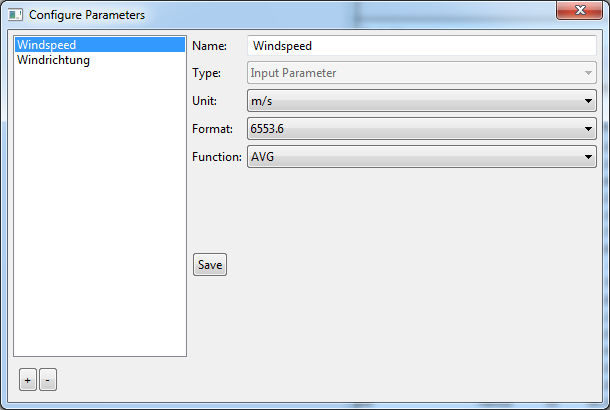
\includegraphics[width=\linewidth]{master/parameters.jpg}
    \caption{Adding/editing of the parameters}
    \label{fig:parameter}
\end{figure} 

\begin{figure}
     \centering 
     \subfloat[Quick overview of the slaves and their status]{\label{fig:main} 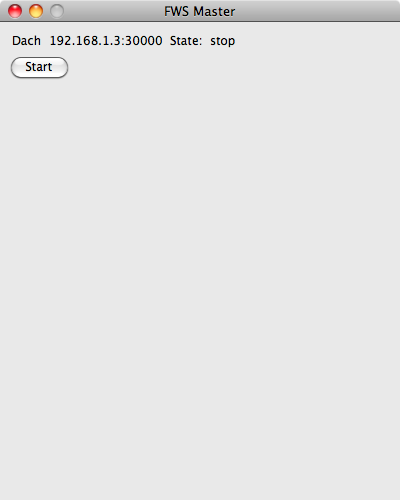
\includegraphics[width=0.4\linewidth]{master/mainview.png}} 
      \qquad
     \subfloat[Configuration of the basic settings]{\label{fig:settings} 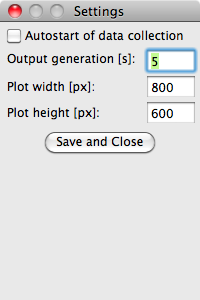
\includegraphics[width=0.4\linewidth]{master/settings.png}}
      \qquad
      \subfloat[Add new Slave]{\label{fig:add} 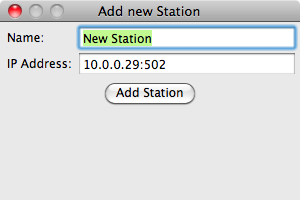
\includegraphics[width=0.4\linewidth]{master/add.png}}
     \caption{Screenshots of FWS Master} 
     \label{view1}
\end{figure}


\begin{figure}[p]
    \centering
    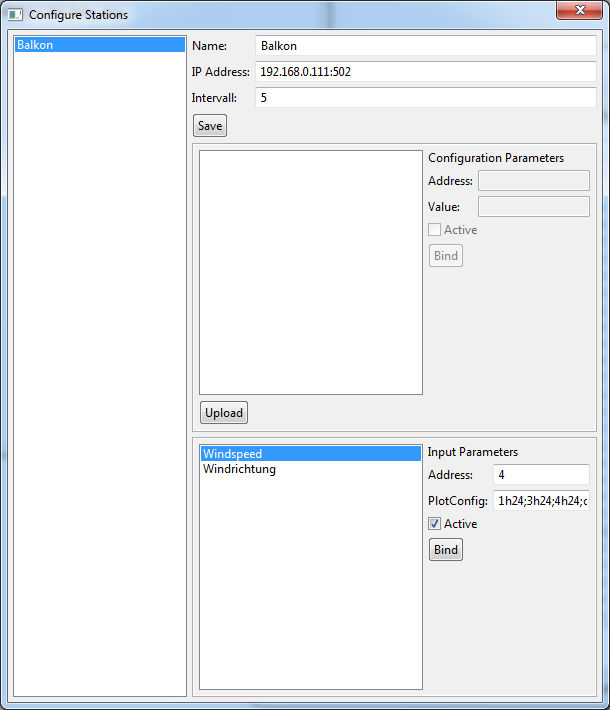
\includegraphics[width=\linewidth]{master/slaves.jpg}
    \caption{Editing slave specific settings. The parameter bindings are also set here}
    \label{fig:slaves}
\end{figure}

\begin{figure}[p]
    \centering
    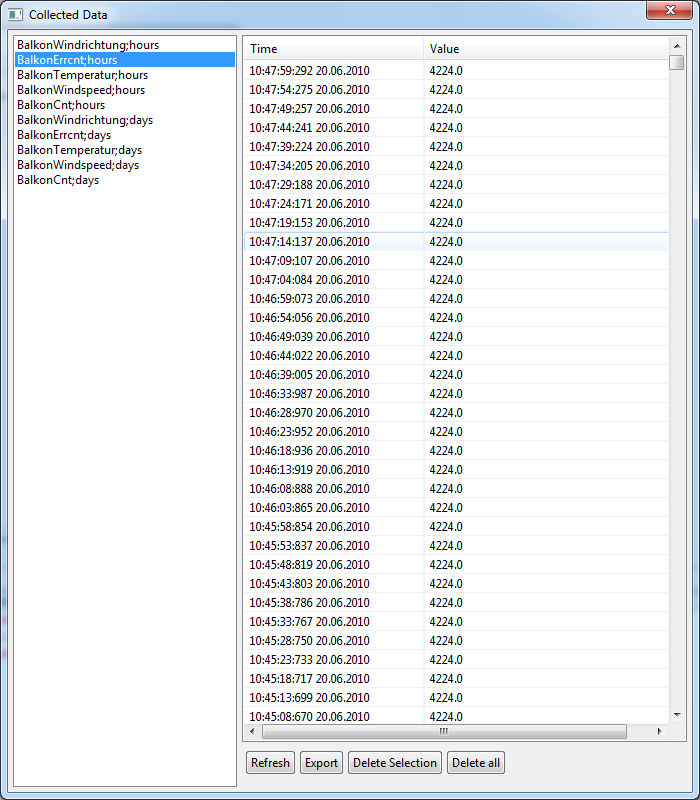
\includegraphics[width=\linewidth]{master/viewdata.jpg}
    \caption{Shows the currently collected and saved data}
    \label{fig:data}
\end{figure}
% subsection screenshots (end)
